%%%%%%%%%%%%%%%%%%%%%%%%%%%%%%%%%%%%%%%%%
% Short Sectioned Assignment
% LaTeX Template
% Version 1.0 (5/5/12)
%
% This template has been downloaded from:
% http://www.LaTeXTemplates.com
%
% Original author:
% Frits Wenneker (http://www.howtotex.com)
%
% License:
% CC BY-NC-SA 3.0 (http://creativecommons.org/licenses/by-nc-sa/3.0/)
%
%%%%%%%%%%%%%%%%%%%%%%%%%%%%%%%%%%%%%%%%%

%----------------------------------------------------------------------------------------
%	PACKAGES AND OTHER DOCUMENT CONFIGURATIONS
%----------------------------------------------------------------------------------------

\documentclass[paper=a4, fontsize=10pt]{article} % A4 paper and 11pt font size

\usepackage[utf8]{inputenc} % Use 8-bit encoding that has 256 glyphs
%\usepackage{fourier} % Use the Adobe Utopia font for the document - comment this line to return to the LaTeX default
\usepackage[english]{babel} % English language/hyphenation
\usepackage{amsmath,amsfonts,amsthm} % Math packages
\usepackage{graphicx}
\graphicspath{ {/home/euan/Desktop/} }
\usepackage{tikz}
\usetikzlibrary{arrows}
\usepackage{algorithm}
\usepackage[noend]{algpseudocode}

\makeatletter
\def\BState{\State\hskip-\ALG@thistlm}
\makeatother



%\usepackage{sectsty} % Allows customizing section commands
%\allsectionsfont{\normalfont \large} % Make all sections centered, the default font and small caps
%\usepackage{tikz}
%\usetikzlibrary{arrows}

%\usepackage{titlesec}
%\titleformat*{\subsubsection}{\bfseries}

\usepackage[margin=1in]{geometry}


%\usepackage{fancyhdr} % Custom headers and footers
%\pagestyle{fancyplain} % Makes all pages in the document conform to the custom headers and %footers
%\fancyhead{} % No page header - if you want one, create it in the same way as the footers below
%\fancyfoot[L]{} % Empty left footer
%\fancyfoot[C]{} % Empty center footer
%\fancyfoot[R]{\thepage} % Page numbering for right footer
%\renewcommand{\headrulewidth}{0pt} % Remove header underlines
%\renewcommand{\footrulewidth}{0pt} % Remove footer underlines
%\setlength{\headheight}{12pt} % Customize the height of the header

\numberwithin{equation}{section} % Number equations within sections (i.e. 1.1, 1.2, 2.1, 2.2 instead of 1, 2, 3, 4)
\numberwithin{figure}{section} % Number figures within sections (i.e. 1.1, 1.2, 2.1, 2.2 instead of 1, 2, 3, 4)
\numberwithin{table}{section} % Number tables within sections (i.e. 1.1, 1.2, 2.1, 2.2 instead of 1, 2, 3, 4)

\setlength\parindent{0pt} % Removes all indentation from paragraphs - comment this line for an assignment with lots of text

%----------------------------------------------------------------------------------------
%	TITLE SECTION
%----------------------------------------------------------------------------------------

\title{Huffman Codes}
\author{Robert T. Lange, Nandan Rao, Euan Dowers}
\date{}

\begin{document}

\maketitle % Print the title

%----------------------------------------------------------------------------------------
%	THE PROBLEM 
%----------------------------------------------------------------------------------------
\section{Prefix Codes}

Given an alphabet $A$ with letters $a \in A$, define a \textit{code}, $c$, as an injective function $c$ where $x$ is replaced by a variable-length binary string $c(x)$\footnote{i.e. $c:A \rightarrow \mathbb{Z}^2_1 \cup \mathbb{Z}^2_2 \cup \ldots \cup \mathbb{Z}^2_n$ for some $n$, and $c(x) = c(y) \Rightarrow x=y$. }. Define a \textit{prefix code} as a code such that for all $x,y \in A$, $x \neq y$, $c(x)$ is not a prefix of $c(y)$. Therefore, given the code $c$ a prefix code can be decoded reading left to right. 
\\
\\
Given a text $T$ that uses an alphabet $A$, for each $x \in A$ let $f_x$ denote the frequency of $x$ in $T$. The average number of bits needed to encode $T$ is therefore given by
%%%%%%%%%%%%
\[
C = \sum _ {x \in A} f_x | c(x) |.
\]
%%%%%%%%%%%%
Our aim is to find a prefix code for $T$ that minimises $C$. This problem was solved by David A. Huffman in 1952, when he was still a Ph.D student \cite{huffman52}. The algorithmic paradigm used is the Greedy Algorithm, by building a binary tree to represent the text $T$, starting with the list of letters in $A$, sorted from low to high by $f_x$, then at each step forming a parent node for the two nodes with the lowest frequency and inserting this parent back into the list with a frequency $f_x + f_y$ and sorting. 
%----------------------------------------------------------------------------------------
%	THE ALGORITHM
%----------------------------------------------------------------------------------------
\section{Algorithm}
\subsection{Encoding}
The algorithm we have implemented in encoding a string, as is common in the literature \cite{huffman52}\cite{mackay} is as follows

\begin{algorithm}[h]
\caption{Huffman Coding Algorithm}\label{alg:huffman}
\begin{algorithmic}[1]
\Procedure{letter count}{text}
\BState \textit{A} $\gets$ letters used in \textit{text}
\BState \textit{list} $\gets$ empty list
\BState for \textit{x} in \textit{A}:
\State add [\textit{x}, number of occurences of \textit{x} in \textit{text}] to \textit{list}
\BState sort \textit{list} by frequency from low to high
\BState nodes $\gets$ elements of \textit{list} represented as leaf nodes
\EndProcedure

\Procedure{Huffman Tree}{nodes}
\BState while lenth of \textit{nodes} $> 1$:
\State parent $\gets$ Tree( \textit{frequency} = \textit{frequency}(\textit{nodes}[1]) + \textit{frequency}(\textit{nodes}[2]), left child =  \textit{nodes}[1], right child = \textit{nodes}[2]
\State remove \textit{nodes}[1] and \textit{nodes}[2]
\State add parent to \textit{nodes}
\State sort \textit{nodes} by frequency from low to high
\EndProcedure

\Procedure{Huffman Code}{nodes}
\BState add \textit{codeword} string of length 0 to only entry of \textit{nodes}
\BState for \textit{node} in \textit{nodes}:
\If {\textit{node} has children}
\State add leftchild(\textit{node}) to \textit{nodes} with \textit{codeword} of \textit{node} + '0'
\State add rightchild(\textit{node}) to \textit{nodes} with \textit{codeword} of \textit{node} + '1'
\EndIf
\BState \textit{code} $\gets$ \textit{node} and \textit{codeword} in \textit{nodes} where \textit{node} represents a letter in \textit{A}.
\EndProcedure

\Procedure{HuffmanEncode}{\textit{text, code}}
\BState for \textit{letter} in \textit{text}:
\BState \textit{codedmessage} $\gets$ string of length 0
\State \textit{codedletter} $\gets$ \textit{code(letter)}
\State \textit{codedmessage} $\gets$ \textit{codedmessage} + \textit{codedletter}
\BState \textbf{RETURN} \textit{codedmessage}
\EndProcedure
\end{algorithmic}
\end{algorithm}

\pagebreak

\subsubsection{Proof of Correctness}

Assume we are given a text $T$ that uses some alphabet $A$ and we wish to find the optimal prefix code for $T$. Note first that any binary code can be represented by a binary tree, and that any prefix code can be represented as a binary tree where every node that corresponds to a letter is a leaf node. The reasoning for this assertion is straightforward: starting from a root node, and appending a '0' for any subsequent left branch, and a '1' for any subsequent right branch, the code for any letter can be represented by the path taken to reach the node corresponding to that letter in our binary tree. Furthermore, since $c$ is a prefix code, we know that for any letter $x$ the codeword $c(x)$ cannot appear as the prefix of another codeword, so $x$ must be a leaf node of our tree. An example of a (clearly suboptimal) prefix code for the text \texttt{hello} is given in Figure \ref{fig:subopt}, which will give a coded message of \texttt{000001110110111}.
%%%%%%%%%%%%%%%%%%%%%%%%%%%%%%%%%%%

\begin{figure}[h]
\centering 

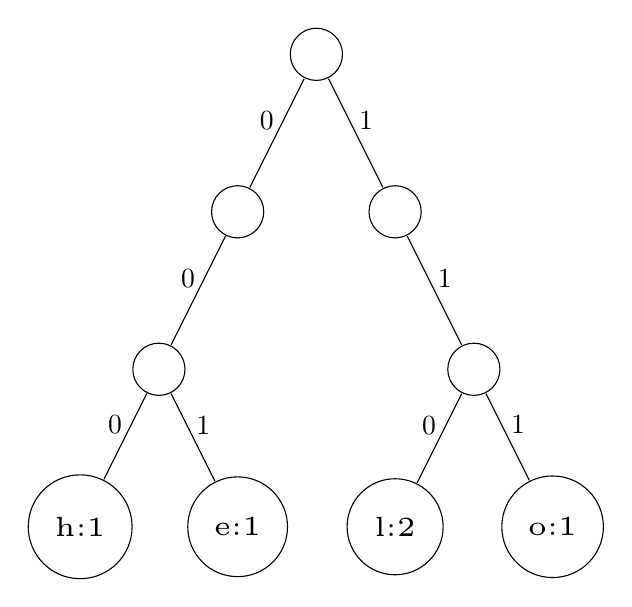
\begin{tikzpicture} [scale=2, every node/.style={scale=2}] 

\tikzset{vertex/.style = {shape=circle,draw,minimum size=0.5em}}
\tikzset{edge/.style = {->,> = latex'}}
% vertices
\node[vertex] (a) at  (4,2) {};
\node[vertex] (b) at  (3.5,1) {};
\node[vertex] (c) at (4.5,1) {};
\node[vertex] (d) at (3,0) {};
\node[vertex] (e) at (5,0) {};
\node[vertex] (f) at (2.5,-1) {\tiny h:1};
\node[vertex] (g) at (3.5,-1) {\tiny e:1};
\node[vertex] (h) at (4.5,-1) {\tiny l:2};
\node[vertex] (i) at (5.5,-1) {\tiny o:1};
%edges
\begin{scope}[every path/.style={-}, every node/.style={inner sep=1pt}]
       \draw (a) -- node [anchor=south east] {0} (b);
       \draw (a) -- node [anchor=south west] {1} (c);
       \draw (b) -- node [anchor=south east] {0} (d);
       \draw (c) -- node [anchor=south west] {1} (e);       
       \draw (d) -- node [anchor=south east] {0} (f);
       \draw (d) -- node [anchor=south west] {1} (g);
       \draw (e) -- node [anchor=south east] {0} (h);
       \draw (e) -- node [anchor=south west] {1} (i);
\end{scope}

\end{tikzpicture}

\caption{Suboptimal prefix code represented as a binary tree} \label{fig:subopt}
\end{figure}
%%%%%%%%%%%%%%%%%%%%%%%%%%%%%%%%%%%

It is clear that any optimal prefix code will not have any redundant digits, as the code in Figure \ref{fig:subopt} does (in the second digit of every codeword). This is equivalent to saying that all nodes other than leaf nodes must have two children. Therefore, any optimal prefix code must follow some kind of bottom-up pairing approach as in Algorithm \textbf{REF}.
\\
\\
At each iteration of the node parenting step in the algorithm described in the previous subsection, the algorithm is essentially adding $f_{(1)} + f_{(2)}$ bits to the length of the final encoded message, where $f_{(i)}$ represents the frequency of the $i$-th least frequent node in our list. Therefore, since we sort the list of available child nodes at the end of each iteration, we are adding the smallest possible length to our encoded message in each iteration.
\\
\\
Therefore, Algorithm \textbf{REF} defines the optimal prefix code defined by such a bottom up pairing algorithm, and since we have shown that any optimal prefix code must be able to be generated by such an algorithm, Algorithm \textbf{REF} defines an optimal prefix code.  

\subsubsection{Complexity}

\subsection{Decoding}

\subsubsection{Proof of Correctness}

\subsubsection{Complexity}




%%%%%%%%%%%%%%%%%%%%%%%%%%%%%%%%%%%%%%%%%%%%%%%%%%%%%%%%%%%
\pagebreak

\begin{thebibliography}{9}
\bibitem{huffman52} 
David A. Huffman. 
\textit{A Method for the Construction of Minimum-Redundancy Codes}. 
Proceedings of the I.R.E. 40(9), 1952.
 
\bibitem{mackay} 
David J.C. MacKay. 
\textit{Information Theory, Inference and Learning Algorithms}. 
Cambridge University Press, 2003.
\end{thebibliography}
 

\end{document}